\documentclass[]{article}
\usepackage{amsmath}
\usepackage{amssymb}
\usepackage{stmaryrd}
\usepackage{latexsym}
\usepackage{graphicx}
\usepackage{fancyhdr}
\usepackage{color}
\usepackage{listings}
\usepackage[top=1in, right=0.75in, left=0.75in]{geometry}
\usepackage[colorlinks=true, linkcolor=blue]{hyperref}

\definecolor{customgreen}{rgb}{0,0.6,0}
\definecolor{customgray}{rgb}{0.5,0.5,0.5}
\definecolor{custommauve}{rgb}{0.6,0,0.8}

\definecolor{dkgreen}{rgb}{0,0.6,0}
\definecolor{gray}{rgb}{0.5,0.5,0.5}
\definecolor{mauve}{rgb}{0.58,0,0.82}

\lstset{frame=tb,
	language=MATLAB,
	aboveskip=3mm,
	belowskip=3mm,
	showstringspaces=false,
	columns=flexible,
	frame=single,	                   % adds a frame around the code
	basicstyle={\small\ttfamily},
	numbers=none,
	numberstyle=\tiny\color{gray},
	keywordstyle=\color{blue},
	commentstyle=\color{dkgreen},
	stringstyle=\color{mauve},
	breaklines=true,
	rulecolor=\color{black},
	breakatwhitespace=true,
	tabsize=3,
	numbers=left,                    % where to put the line-numbers; possible values are (none, left, right)
	numbersep=10pt,                   % how far the line-numbers are from the code
	numberstyle=\tiny\color{customgray}, % the style that is used for the line-numbers
}

\author{
	Mohammad Hossein Shafizadegan\\
	99104781
}
\title{
	Assignment 2 \\
	Computational Intelligence  \\
	Dr. S. Hajipour
}

\pagestyle{fancy}
\rhead{CI}
\lhead{Assignment 2}

\newcommand{\pict}[2]{\begin{center}
		\includegraphics[width=#1\linewidth]{Fig/#2.png}
\end{center}}
\newcommand{\mat}[1]{\begin{bmatrix} #1 \end{bmatrix}}
\newcommand{\deter}[1]{\begin{vmatrix} #1 \end{vmatrix}}

\definecolor{customgreen}{rgb}{0,0.6,0}
\definecolor{customgray}{rgb}{0.5,0.5,0.5}
\definecolor{custommauve}{rgb}{0.6,0,0.8}

\begin{document}
	\begin{figure}
		
\includegraphics[width=0.25\textwidth]{Fig/Sharif.png}
		\centering
	\end{figure}
	\maketitle
	\tableofcontents
	\newpage
		%-----------------------------------------------------------------------------------------------------------------	
	\section{Question 1}
	\subsection*{a}
	\pict{0.6}{F1}
	Regarding the above figure, demonstrating the curve for the original, common error function and the new defined one, it is quite vivid that the original error function has an unlimited range and can be increased unlimited but the values of the new defined error function varies between 0 and 1. Indeed this function will somehow normalize the error and map great errors to one using a kind of threshold which is defined by the value of $\sigma$. 
	\pict{0.6}{F2}
	Also it cab be seen that using this new error function we will deal with a smoother function.
	\subsection*{b}
	\begin{flalign*}
		&\nabla_{W_u} \, e^{(l)} = \frac{\partial \, e^{(l)}}{\partial W_u} = \frac{\partial \, e^{(l)}}{\partial net_{u}^{(l)}} \, \frac{\partial net_{u}^{(l)}}{\partial W_{u}} \qquad , \qquad \frac{\partial net_{u}^{(l)}}{\partial W_{u}} = in_u^{(l)}&&\\\\
		&\frac{\partial \, e^{(l)}}{\partial net_{u}^{(l)}} = \sum_{v\in U_{out}} \frac{\partial e_v^{(l)}}{\partial net_u^{(l)}} = \begin{cases}
			-\sum_{v\in U_{out}} \frac{\pi\sin\left(\frac{\pi(o_v^{(l)} - out_v^{(l)} )^2}{2\sigma}\right)(o_v^{(l)} - out_v^{(l)})}{2\sigma} \, \frac{\partial out_v^{(l)}}{\partial net_u^{(l)}} \quad & (o_v^{(l)} - out_v^{(l)})^2 < 2\sigma \\\\
			\qquad 0 & O.W.
		\end{cases}&&\\\\
		&\forall u \in U_{out} \, : \, \delta_u^{(l)} = \sin\left(\frac{\pi(o_v^{(l)} - out_v^{(l)} )^2}{2\sigma}\right)(o_v^{(l)} - out_v^{(l)}) \, \frac{\partial out_v^{(l)}}{\partial net_u^{(l)}}&&
	\end{flalign*}
	\begin{flalign*}
		&\forall u \in U_{out} \, : \, \nabla_{W_u} e_u^{(l)} = \frac{\partial e_u^{(l)}}{\partial W_u} = \frac{\partial \, e^{(l)}}{\partial net_{u}^{(l)}} \, \frac{\partial net_{u}^{(l)}}{\partial W_{u}} = -\frac{\pi}{2\sigma} \sin\left(\frac{\pi(o_v^{(l)} - out_v^{(l)} )^2}{2\sigma}\right)(o_v^{(l)} - out_v^{(l)}) \, \frac{\partial out_v^{(l)}}{\partial net_u^{(l)}} \, in_u^{(l)}&&\\
		&\Delta W_u^{(l)} = -\frac{\eta}{2} \nabla_{W_u} e_u^{(l)} = \frac{\pi\eta}{4\sigma} \sin\left(\frac{\pi(o_v^{(l)} - out_v^{(l)} )^2}{2\sigma}\right)(o_v^{(l)} - out_v^{(l)}) \, \frac{\partial out_v^{(l)}}{\partial net_u^{(l)}} \, in_u^{(l)}&&
	\end{flalign*}

		%-----------------------------------------------------------------------------------------------------------------	
	\section{Question 2}
	\subsection*{a}
	\textbf{Overfitting} occurs when a model is too complex and fits the training data too closely, capturing not only the underlying pattern but also the random noise and fluctuations. As a result, the model performs well on the training data, but poorly on the testing data or any new data from the same problem domain. Overfitting indicates that the model has low bias but high variance, meaning that it is very sensitive to changes in the training data.\\\\
	\textbf{Underfitting} occurs when a model is too simple and fails to capture the underlying pattern of the data. The model performs poorly on both the training and testing data, indicating that it has high bias but low variance, meaning that it is not able to represent the true relationship between the input and output variables accurately.\\\\
	Based on the provided figures, it can be seen vividly that we are facing \textbf{overfitting} in the first figure as the fitted line is a complex polynomial with lots of features. The second model is quite well-fitted. Its not complex and meanwhile not too simple. The third figure represents an underfitted model as it is too simple which can't represent the behavior of the data.
	\pict{0.7}{F3} 
	
	\subsection*{b}
	While we are suffering from overfitting, the error for training set will be zero or very close to zero. As we know in this case the model has no generalization and it seems like it has memorize the training data. \\\\
	On the flip side the error for test and evaluation data will be high as there is no generalization for the model which is overfitted.
	
	\subsection*{c}
	In the provided figure the x axis stands for the complexity of the model.\\\\
	The red colored curve represents the error for evaluation or test data. As it can be seen that in the beginning, the error rate will decrease by making the model more complex but after a particular level of complexity, the more complex the model is, the higher error we have.\\\\
	The blue colored curve represents the error rate for training data. Even when the model is overfitted, the training data will continue decreasing.\\\\
	The point at which the evaluation error starts to increase (which indeed, is marked by the green vertical line) is the level of complexity that the overfitting has occurred.
	
	\pict{0.4}{F4}
	
	\subsection*{d}
	Here some common methods to avoid underfitting in perceptron neural networks:
	\begin{itemize}
		\item Increase the number of hidden layers and neurons in the network, to increase its capacity and complexity.
		\item Increase the number of features or perform feature engineering, to provide more relevant and informative input data to the network.
		\item Increase the number of features or perform feature engineering, to provide more relevant and informative input data to the network. Feature engineering can be achieved by creating new features or transforming existing features.
		\item Increase the number of epochs or the duration of training, to allow the network to learn more from the data.
	\end{itemize} 

	\subsection*{e}
	K-fold cross-validation involves splitting the dataset into k equal-sized subsets or folds, and using one fold as the validation set and the rest as the training set. The model is trained on the training set and tested on the validation set, and the process is repeated k times, each time using a different fold as the validation set.\\\\
	This technique is useful for preventing underfitting specially when we lack enough data for training process. By using different folds as the validation and training set, k-fold cross-validation ensures that the model is trained and tested on all the data and not just a specific subset. 
	
		%-----------------------------------------------------------------------------------------------------------------	
	\section{Question 3}
	Based on the provided information, \textbf{sensitivity} is the priority in this case.\\\\
	Sensitivity indicates the ability to correctly identify individuals as sick or positive. In this scenario, if a person is sick and mistakenly labeled as healthy, it can lead to high costs and serious risks for them. Therefore, more importance is given to sensitivity to ensure that patients are correctly identified and receive appropriate treatment.\\\\
	On the other hand, the false positive error, which refers to mistakenly diagnosing a healthy person as sick, can be also important. However, in this context, if a healthy person is mistakenly identified as sick, it may incur higher financial costs but generally has less impact on individuals' health.\\\\
	Therefore, considering these explanations, sensitivity takes precedence to ensure that patients are correctly identified and receive appropriate treatment
	
		%-----------------------------------------------------------------------------------------------------------------	
	\section{Question 4}
	\begin{flalign*}
		&\frac{\partial \, e}{\partial W_{ab}} = \frac{\partial \, e}{\partial net_{b}} \, \frac{\partial net_{b}}{\partial W_{ab}}&&\\
		&\frac{\partial \, e}{\partial net_{b}} = \frac{\partial e}{\partial \log(out_b)} \, \frac{\partial \log(out_b)}{\partial net_{b}} \qquad , \qquad out_i = f_{act_i} \Rightarrow \log(out_b) = net_b - \log\left(\sum_{j=1}^{m} e^{net_j}\right) &&\\
		&\frac{\partial \log(out_b)}{\partial net_{b}} = 1 - \frac{e^{net_b}}{\sum_{j=1}^{m} e^{net_j}} \quad \Rightarrow \quad \frac{\partial \, e}{\partial net_{b}} = -o_b \left(1 - \frac{e^{net_b}}{\sum_{j=1}^{m} e^{net_j}}\right) =  out_b - o_b&&\\
		&\frac{\partial net_{b}}{\partial W_{ab}} = in_a \quad \Rightarrow \quad \frac{\partial \, e}{\partial W_{ab}} = in_a(out_b - o_b) \qquad \Rightarrow \qquad \Delta W_{ab} = -\frac{\eta}{2} \, \frac{\partial \, e}{\partial W_{ab}} = -\frac{\eta}{2} \, in_a(out_b - o_b)&&
	\end{flalign*}

		%-----------------------------------------------------------------------------------------------------------------	
	\section{Question 5}
	In our MLP network, we define the network function as weighted summation of inputs, the activation function as step function and the output function as identity function.\\\\
	We require $N^2$ input neurons, each representing a cell of the chess board.\\\\
	We design separate networks for checking rows, columns and diagonals correspondingly. Then at the end, we perform logical "AND" on the results of these three networks to determine the final output of the network and solution to the problem.\\\\
	In each row and column we want to have only one queen. Therefor, only one cell must be 1 and other must be 0. Using sum of products term, the logical function will be as follows:
	\begin{align*}
		x_1 \, \overline{x_2} \, \overline{x_3} \, \dots \, \overline{x_N} + \overline{x_1} \, x_2 \, \overline{x_3} \, \dots \, \overline{x_N} + \dots + \overline{x_1} \, \overline{x_2} \, \overline{x_3} \, \dots \, x_N
	\end{align*} 
	The process is quite the same for the diagonals but we have to use cells located on the diagonals as inputs for our SOP terms.\\\\
	Finally in order to complete the design of the network, we remember that AND and OR functions are implemented as follows:
	\begin{align*}
		\text{AND : } w_i = \begin{cases}
			2 \qquad & \text{ if } l_i = x_i \\
			-2 & \text{ if } l_i = \overline{x_i}
		\end{cases} \qquad , \qquad \theta = n - 1 + \frac{1}{2} \sum_{i=1}^{n} w_i \qquad , \qquad \text{ OR : } w_i = 2 \quad , \quad \theta = 1
	\end{align*}
	Regarding what we explained above, the network specifications are fully determined.
	
		%-----------------------------------------------------------------------------------------------------------------	
	\section{Question 6}
	\subsection*{a}
	Based in the provided figure b in the question, we want to implement the following function using a MLP network
	\begin{align*}
		f(x,y) = \begin{cases}
			f_{11} = 2 \qquad & 0<x<5 \,\, , \,\, 0<y<5\\
			f_{12} = 4  & 0<x<5 \,\, , \,\, 5<y<10\\
			f_{21} = 6 & 5<x<10 \,\, , \,\, 0<y<5\\
			f_{22} = 8  & 5<x<10 \,\, , \,\, 5<y<10
		\end{cases}
	\end{align*}
	The architecture of the network is as follows:
	\begin{itemize}
		\item \textbf{Input:}\\
		Two input neurons for $x$ and $y$.
		\item \textbf{Layer 1:}\\
		We design a layer to check if $x$ and $y$ are less or greater than 5. This layer contains two neurons
		\item \textbf{Layer 2:}\\
		Using 4 neurons which implement logical AND, we determine which zone of the defined four sections are the specific $x$ and $y$ are belongs to.
		\item \textbf{Output:}\\
		One neuron is required. The weights for this neuron are the defined values assigned for each section correspondingly. We note that this neuron has one hot input.
	\end{itemize}
	We note that the network function for all neurons is the weighted summation and the activation function is sigmoid step function except for the output neuron which has an identity function. and the output function is the identity function. The resulting network can be seen below:
	\pict{0.5}{F12}
	
	\subsection*{b}
	The idea which can be useful for this question is to first recognize which region has the greater error value, then we try to enhance our estimation by dividing that region into more sections. In a loop, we repeatedly perform the same process. Every time we create new sections we have to add some neurons e.g. 2 ones to create 4 new subsections. Also in each step we need some neurons to determine which region has the greater error value.
	
		%-----------------------------------------------------------------------------------------------------------------	
	\section{Question 7}
	\subsection*{a}
	A valid sequence is a one which doesn't contain similar numbers. In order to design the MLP network, the number of required input neurons is equal to number of the cities. In the next layer, we check each two cities to see if they are equal or not. To do so we use a MLP sub-unit which implements biimplication (figure below). 
	\pict{0.4}{F13}
	We use this sub-unit for all different combinations of two cities and finally in the output layer, we use logical OR function two determine the final output of the MLP network.\\\\
	Note that the neurons used in this network have weighted sum network function, step function as the activation function and the output function is identity function.
	
	\subsection*{b}
	In order to find out how many cities the seller hasn't traveled to, we can use the similar cities in the sequence. The number of untraveled cities equals to number of similar pairs in the given sequence.\\\\
	To design the network, we use the one we implemented in the previous section. The only thing we have to do is to add the inputs of the output neuron instead of performing the logical OR function. To do so the activation function of the output neuron must defined as identity function instead.
	
	\subsection*{c}
	We need 14 input neurons to process the $x$ and $y$ coordinates of the cities. Then we process the $x$ coordinates with each other to calculate the $|x_i - x_j|$. The same process will be done for $y$ coordinates and finally using an output layer similar to the one we used in the previous section which adds $|x_i - x_j|$ and $|y_i - y_j|$ for adjacent cities in order to find the total traveled distance.\\\\
	The network we design for calculating the $x$ and $y$ distance can be seen below:
	\pict{0.7}{F14}
	
		%-----------------------------------------------------------------------------------------------------------------	
	\section{Question 8}
	First we find a way to encode the movement of the robot using binary coding.
	\begin{center}
		\begin{tabular}{|c|c|c|}
			\hline
			Movement & $o_1$ & $o_2$ \\ \hline
			Front & 0 & 0\\
			Left & 0 & 1 \\
			Right & 1 & 0\\
			$180^\circ$ rotation & 1 & 1\\
			\hline
		\end{tabular}
	\end{center}
	The inputs ($x_i$) are used to determine the existence of obstacles in left, front and right. Using this coding, we create the following table as decision policy for the robot.
	\begin{center}
		\begin{tabular}{|c|c|c||c|}
			\hline
			$x_1$ & $x_2$ & $x_3$ & direction \\ \hline
			1 & 1 & 0 & right\\
			0 & 1 & 1 & left \\
			0 & 1 & 0 & right\\
			1 & 0 & 1 & front\\
			0 & 0 & 1 & front \\
			1 & 0 & 0 & front \\
			1 & 1 & 1 & $180^\circ$ turn \\
			\hline
		\end{tabular}
	\end{center}
	Now using sum of product term we simply implement and design the network using AND and OR units which we already now how to design them.\\\\
	For all the neurons of this network we use weighted sum as network function, step function as activation and identity function as output.
		%-----------------------------------------------------------------------------------------------------------------	
	\section{Question 9}
	\subsection*{a}
	First we define the vector $x$ and then we simply plot the provided cost function using the following code.
	\begin{lstlisting}
		dx = 0.01;
		x = -0.2:dx:4.2;
		
		f = @(x) 5/6 * x.^4 - 7*x.^3 + 115/6 * x.^2 - 18.*x + 6;
		
		figure;
		plot(x, f(x), 'linewidth', 2);
		title('Cost function')
		xlabel('x');
		ylabel('f(x)')
	\end{lstlisting}
	The resulting curve can be seen below:
	\pict{0.45}{F5}
	
	\subsection*{b}
	In order to implement the gradient descent algorithm, we first have to define the function and the derivative of the function using a symbolic variable. The code for this section is as follows:
	\begin{lstlisting}
		syms x;
		fx = 5/6 * x.^4 - 7*x.^3 + 115/6 * x.^2 - 18.*x + 6;
		df = matlabFunction(diff(f, x));
	\end{lstlisting}
	Then as it was stated, we calculate the initial value of the $x$ following a gaussian distribution with mean of 2.05 and variance of 1. We also define the parameters of the algorithm including the learning rate and the maximum number of iteration for ending the process.
	\begin{lstlisting}
		avg = 2.05;
		init_x = randn() + avg;
		
		learningRate = 0.02;
		n_iter = 100;
	\end{lstlisting}
	As the main part of the algorithm, in a for loop, we calculate the value of derivative in the specific point and update the value of x in each iteration. At the end of the loop, we check for the finishing and ending conditions. The implemented code for this section is provided below:
	\begin{lstlisting}
		% Perform gradient descent
		x = init_x;
		for i = 1:n_iter
			
			df_val = df(x);
			% Update the current point using the derivative and learning rate
			x = x - learningRate * df_val;
			
			% Check for convergence (i.e., when the derivative is close to zero)
			if abs(df_val) < 1e-2
				break;
			end
		end
		
	\end{lstlisting}
	The results of running this algorithm can be seen here:
	\pict{0.9}{F6}
	Now we want to repeat the same process for different values of learning rate. In order to obey clean code rules, we have developed a function called "gradient\_discent" which insists of the exact previous code. It receives the initial value of $x$, learning rate and other required parameters as input arguments. The outputs of this function are the number of iteration the process took along, the final value of $x$ and the value of the minimum point.\\\\
	Now we run the algorithm for the different values of eta provided using the following code :
	\begin{lstlisting}
		eta = [0.01, 0.02, 0.04, 0.08, 0.1];
		avg = 2.05;
		max_iter = 100;
		
		for i=1:length(eta)
		
			init_x = randn() + avg;
			
			[n_iter, min_x, min_v] = gradient_descent(init_x, eta(i), max_iter, f);
			
			% Display the final result
			disp(['Learning rate = ', num2str(eta(i))])
			disp(['The initial value: x = ', num2str(init_x)])
			disp(['Number of iterations: ', num2str(n_iter)])
			disp(['Minimum point: x = ', num2str(min_x)]);
			disp(['Minimum value: f(x) = ', num2str(min_v)]);
			disp('-----------------------------')
		
		end
		
	\end{lstlisting}
	Here are the results:
	\begin{center}
		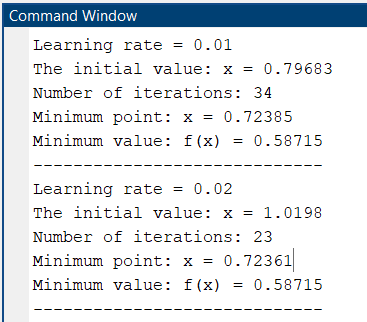
\includegraphics[width=0.25\linewidth]{Fig/F7.png}
		\qquad
		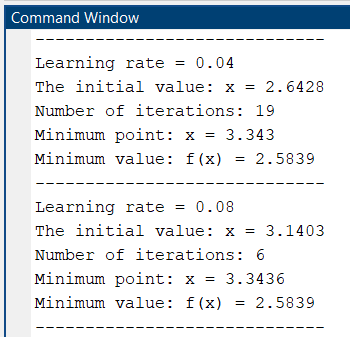
\includegraphics[width=0.23\linewidth]{Fig/F8.png}
		\qquad
		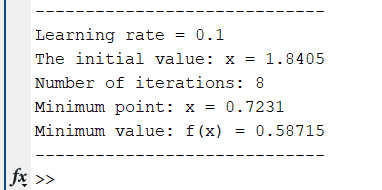
\includegraphics[width=0.25\linewidth]{Fig/F9.png}
	\end{center}
	
	\subsection*{c}
	We first find the global minimum of the cost function using MATLAB builtin function.
	\begin{lstlisting}
		global_min = min(f(x));
	\end{lstlisting}
	Then we have defined an array for storing the probability of reaching the global minimum point.
	\begin{lstlisting}
		prob = zeros(1, length(eta));
	\end{lstlisting}
	Then for each value of learning rate, we use the gradient descent algorithm for $N$ times and then we find the number of times that we have reached the global minimum point for different value of initial point. Hence the probability will be simply calculated by dividing the calculated value by $N$. We note that in order to have a more accurate estimation of the probability we have to set the value of $N$, large enough.
	\begin{lstlisting}
		for i=1:length(eta)
		
			N = 200;
			n_true_min = 0;
			
			for j=1:N
				init_x = randn() + avg;
				[n_iter, min_x, min_v] = gradient_descent(init_x, eta(i), max_iter, f);
				if abs(min_v - global_min) < 1e-5
				n_true_min = n_true_min + 1;
				end
			end
			
			prob(i) = n_true_min / N;
			
		end
	\end{lstlisting}
	Finally we visualize the results.
	\begin{lstlisting}
		figure;
		bar(eta, prob)
		xlabel('eta')
		ylabel('Probability')
		title('Probability of reaching the global min')
		xlim([-0.05 0.105])
		ylim([0 1])
	\end{lstlisting}
	The final results and the asked plot can be seen below:
	\pict{0.4}{F10}
	\subsection*{d}
	In this section in order to observe the effect of the average used for generating the random initial value, we will fix the learning rate to $\eta = 0.02$ and sweep over values of the average.
	\begin{lstlisting}
		global_min = min(f(x));
		avg = 0:0.5:4;
		prob = zeros(1, length(avg));
		eta = 0.02;
		max_iter = 200;
		
		for i=1:length(avg)
		
			N = 100;
			n_true_min = 0;
			
			for j=1:N
				init_x = randn() + avg(i);
				[n_iter, min_x, min_v] = gradient_descent(init_x, eta, max_iter, f);
				if abs(min_v - global_min) < 1e-5
					n_true_min = n_true_min + 1;
				end
			end
			
			prob(i) = n_true_min / N;
			
		end
	\end{lstlisting}
	The result can be seen below:
	\pict{0.4}{F11}
	As it can vividly seen, when we use larger value of average for generation of the initial value of $x$, the chance of having that initial value closer to the global minimum and farther than the local minimum increases which results in a higher chance of reaching the global minimum.
	
	\subsection*{e}
	For this section, in order to check whether the algorithm has converged or not, we have modified the function we implemented before for the gradient descent by adding another output called "flag" which demonstrates the convergence. The flag 0 is equivalent as not converging.\\\\
	We note that for this section, we have fixed the value of the average and we will see how different values of learning rate affect the convergence.
	\begin{lstlisting}
		eta = [0.01, 0.02, 0.04, 0.08, 0.1, 0.15, 0.2, 0.4];
		global_min = min(f(x));
		avg = 2.05;
		prob = zeros(1, length(eta));
		max_iter = 100;
		
		for i=1:length(eta)
		
			N = 50;
			n_diverge = 0;
			
			for j=1:N
				init_x = randn() + avg;
				[n_iter, min_x, min_v, flag] = modified_gradient_descent(init_x, eta(i), max_iter, f);
				if ~flag
					n_diverge = n_diverge + 1;
				end
			end
			
			prob(i) = n_diverge / N;
		
		end
		
		figure;
		bar(eta, prob)
		xlabel('eta')
		ylabel('Probability')
		title('Probability of divergence')
		xlim([-0.02 0.45])
		ylim([0 1])
		
	\end{lstlisting}
	
	The results can be seen below:
	\pict{0.4}{F15}
	The above results have been achieved using $max\_iter = 50$ which is relatively small value. It is vivid that for larger amount of learning rate, the probability of divergence increases as well.
	
\end{document}